% !TeX spellcheck = en_US
\chapter{Approach}\label{ch:approach}

This chapter contains the solution approaches to the parts of the thesis. Firstly, a formal model of a compressor is defined. Based on that, the key performance indicators which will be used to measure the performance of the single compressors are introduced. Secondly, the two existing compressors HDT and GRP are compared. Finally, improvements of the compression will be suggested.


\section{Compressor Models}

Here, two compressor models will be introduced, one for general compressors and another one for RDF compressors. 

\subsection{General Compressor Model}\label{sec:generalcompressorModel}

\begin{figure}
	\centering
	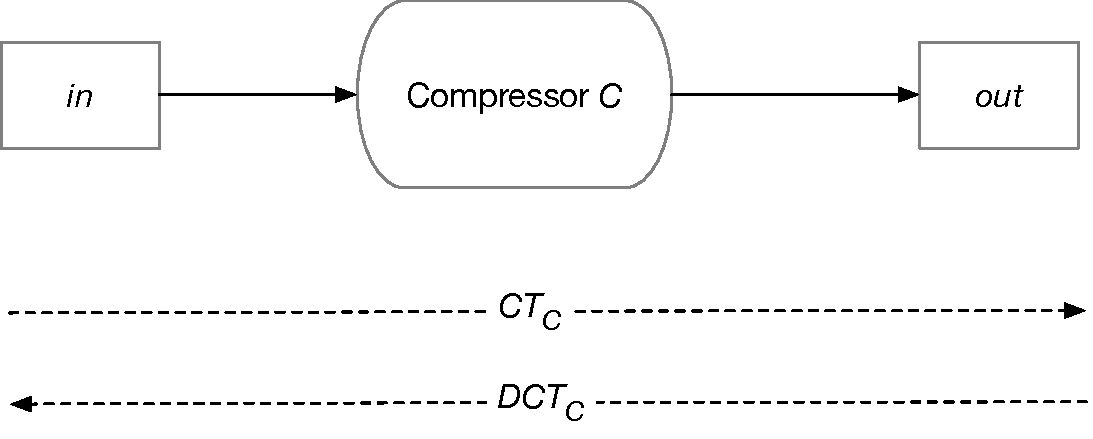
\includegraphics[width=0.8\linewidth]{figures/approach/model_general}
	\caption{Visualization of the General Compressor Model.}
	\label{fig:generalcompressorModel}
\end{figure}

A general purpose compressor $C$ can be described as follows: $C$ takes an input $in$ and produces an output $out$. That step is called compression. Decompression can be described as taking $out$ as an input and producing $in$. An illustration can be seen in Fig.~\ref{fig:generalcompressorModel}. The terms $CT_C$ and $DCT_C$ denote the time for compression and decompression, respectively. They will be explained in more details in Ch.~\ref{sec:approachComprTime}.

An example for a general compressor is GZip~\footnote{https://www.gzip.org/} which will be used in Ch.~\ref{sec:evaluationFinal} as a baseline for GRP and HDT.

\subsection{RDF Compressor Model}\label{sec:compressorModel}

This chapter introduces a formal model for an RDF compressor which can be seen as a sub class or extension of the general model in Ch.~\ref{sec:generalcompressorModel}. It is illustrated in Fig.~\ref{fig:compressorModel}. Here, the compressor $C$ is more complex, as it consists of two components. The first one is called $Dict_C$ and it handles the dictionary compression. That mechanism has already been introduced in the context of HDT (see Ch.~\ref{related_work_hdt}). It assigns an ID to each URI, literal or blank node ID of the graph and can then also further compress the dictionary (like in HDT with prefix trees). The result of $Dict_C$ is $out_{dict}$ which is displayed in the right of Fig.~\ref{fig:compressorModel}. 

The IDs created by $Dict_C$ are then delivered to the second component, $Graph_C$, which is responsible for compressing the RDF graph. It only uses the IDs from $Dict_C$ and does not know about the URIs, literals and blank node IDs. Its result is called $out_{graph}$ which, together with $out_{dict}$, forms the complete output $out$ ($out=\{out_{dict}, out_{graph}\} $). $out_{graph}$ and $out_{dict}$ can each be a single file or a set of files. 

\begin{figure}
	\centering
	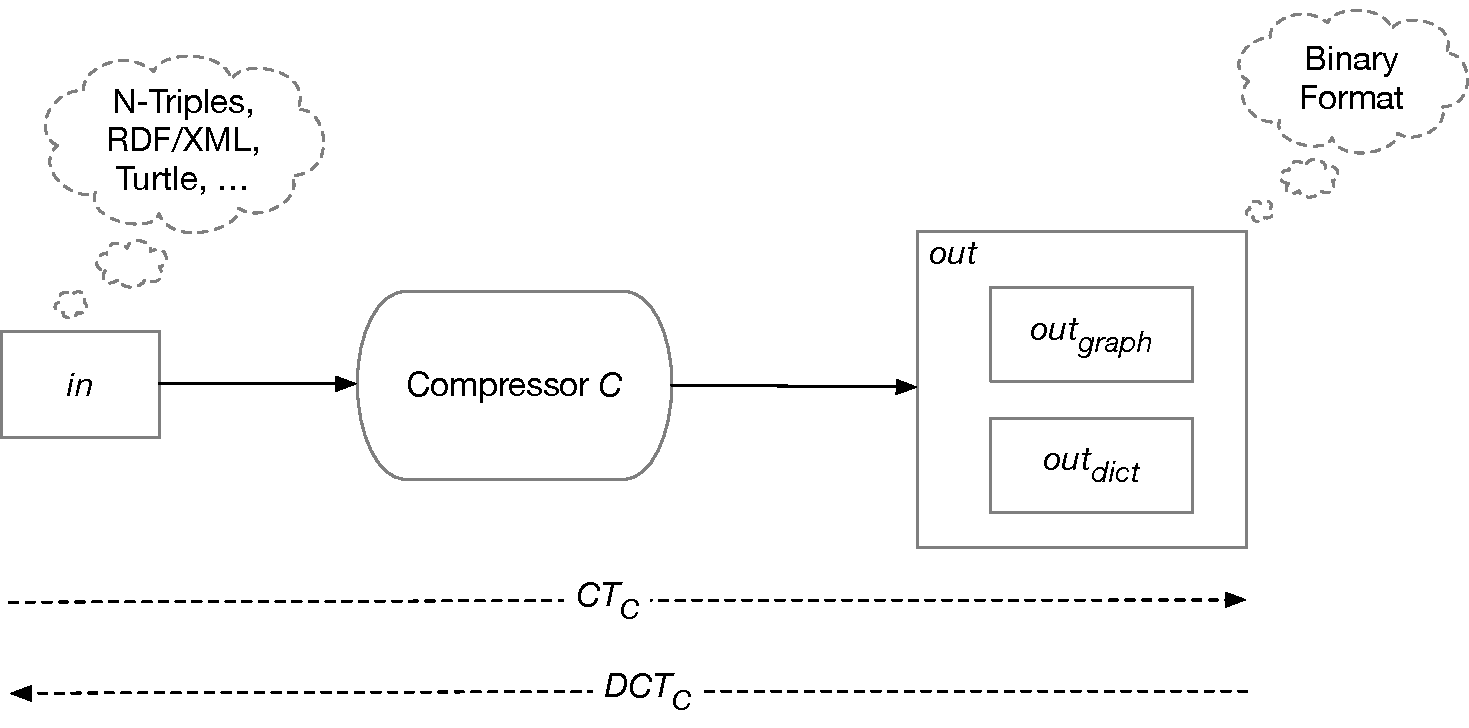
\includegraphics[width=\linewidth]{figures/approach/model}
	\caption{Visualization of the RDF Compressor Model.}
	\label{fig:compressorModel}
\end{figure}


\subsection{Existing RDF  Compressors}

Tab.~\ref{tab:compressorsOverview} shows an overview of the RDF compressors discussed in this thesis and in which way they fulfill the model from Ch.~\ref{sec:compressorModel}. As already explained in Ch.~\ref{related_work_hdt}, $Dict_{HDT}$ assigns IDs and compresses the dictionary. In contrast, $Dict_{GRP}$  only assigns IDs and omits the dictionary afterwards. $Dict_{GRP}$ is therefore not a real dictionary compressor. We solve this problem by replacing  $Dict_{GRP}$ with $Dict_{HDT}$. This way, comparing HDT and GRP in a fair way is possible. It must also be mentioned that $Graph_{HDT}$ includes the HDT header (see Ch.~\ref{related_work_hdt}). Even if the header is not needed for decompression, its size will be part of $out_{graph}$. But this is not a problem, because the header's size is so small that it does not add a significant amount to $out_{graph}$.

\begin{center}
	\begin{tabular}{|c|c|c|}
		\hline 
		& $Dict_{C}$ & $Graph_{C}$ \\ 
		\hline \hline
		HDT & $\checkmark$ & $\checkmark$  \\ 
		\hline 
		GRP & only ID assignment (no storage of $out_{dict}$) & $\checkmark$ \\ 
		\hline 
	\end{tabular} 
	\captionof{table}{Overview of RDF compressors presented in this thesis.}	
	\label{tab:compressorsOverview}
\end{center}

\section{Key Performance Indicators}

In this chapter, key performance indicators for general and RDF compressors are introduced. Those indicators will be measured in order to determine the overall performance of the different compressors.

\subsection{Compression Ratio}

One of the key performance indicators for a compressor $C$ is its compression ratio. Let $m$ be a single file or a set of files. Then $|m|$ is defined as the size which is measured in bytes. The compression ratio is defined by the following equations:

\begin{align}
CR_{C} = \dfrac{|out|}{ |in|} \label{eq:complete}
\end{align}

\begin{align}
CR_{Dict_C} = \dfrac{|out_{dict}|}{ |in|} \label{eq:dict}
\end{align}

\begin{align}
CR_{Graph_C} = \dfrac{|out_{graph}|}{ |in|} \label{eq:graph}
\end{align}

Eq.~\ref{eq:complete} defines the compression ratio for the whole output $out$. Therefore, it is applicable to general and RDF compressors.

In contrast, Eq.~\ref{eq:dict} and~\ref{eq:graph} define the compression ratio only with regard to $out_{dict}$ or $out_{graph}$, respectively. They are only applicable for RDF compressors, since a general compressor has no distinction between $out_{dict}$ and $out_{graph}$. In some cases, it is of interest to only consider either the dictionary or graph compression.

Sometimes, $CR$ is used instead of $CR_C$ if it is clear from the context, which compressor $C$ is considered.

As shown in Fig.~\ref{fig:compressorModel}, $in$ can have different formats. That has to be taken into account with regard to $CR$ as those formats implicate different input sizes. When $CR$ of two compressors is compared, their input has to have the same format.

\subsection{(De-)Compression Time}\label{sec:approachComprTime}

Another key performance indicator of a compressor $C$ is its compression time ($CT_C$) and decompression time ($DCT_C$). These metrics also depend on the input data and indicate the run time needed for compression and decompression of the data, respectively. The run time is typically measured in milliseconds. $CT_C$ and $DCT_C$ are also shown in Fig.~\ref{fig:generalcompressorModel} and~\ref{fig:compressorModel}. They are defined the same for general compressors and RDF compressors. Furthermore, $CT_C$ and $DCT_C$ are only measured for the whole compressor $C$, not for $Dict_C$ or $Graph_C$.

Analogously to $CR$, if is clear from the context which compressor is considered, $CT$ and $DCT$ are used instead of $CT_C$ and $DCT_C$, respectively.


\section{GRP vs HDT}\label{sec:approachGRPvsHDT}

In this chapter, the two existing compressors - HDT and GRP - will be compared. Therefore, the features of the compressors and their applicability to certain features of RDF graphs are discussed.

The question is whether there are certain features that an RDF graph can have, and which have a positive or negative impact on the compression ratio of one or both algorithms. 

As HDT and GRP use the same method for compressing the dictionary ($Dict_{HDT}$), we only compare $Graph_{HDT}$ and $Graph_{GRP}$ in this chapter.

%\subsection{Relation Between Structure of Data and Compression Ratio}\label{sec:relationDataStructureComprRatio}

%Now, it is discussed how the structure of the input graph $in$ influences the compression ratios ($CR_{Graph_C}$) for GRP and HDT. In order to realize that it is necessary to first introduce the star pattern.

\subsection{Star Pattern}\label{sec:approachStarPattern}

According to~\cite{stargraph}, a star is a graph in which one node is connected to all other nodes. The other nodes are not connected to each other. While a star is an extreme case, there exist graphs with a few nodes having very high degrees. We denote them to be similar to the star pattern. 

In order to measure that we define the Star Pattern Similarity ($SPS$). Let $deg(n)$ be the degree of a node $n$. Let $N$ be a list of all nodes sorted by their $deg$-values in descending order.  Let $N_{top}$ be the first $x$ nodes of $N$. Hence, $N_{top}$ contains $x$ nodes with the highest degrees. $x$ should be chosen related to the size of $N$, we choose $x=0.001 \times |N|$.  Then, $SPS$ is defined as follows:

\begin{align*}
SPS=\dfrac{\sum_{n \in N_{top}} deg(n)  }{\sum_{n \in N} deg(n)} \in [0,1]
\end{align*}

The higher the value of $SPS$ is, the more similar the graph is to the star pattern, because then there a few nodes having a high proportion of the sum of all degrees.

The star pattern can be further divided into the hub and authority patterns. As the name suggests, the hub pattern corresponds to a graph in which a few nodes have very high outgoing degrees, the authority pattern is the opposing case (high ingoing degrees). That distinction is needed in the following chapter.

\subsection{HDT}

Next, HDT's behavior with respect to the input is discussed. As HDT's way of compressing the graph structure is fairly simple compared to GRP, there do not seem to be many potential features of the input data that have a high impact on HDT's compression ratio. But one feature is clearly visible: When Fig.~\ref{fig:hdt_overview} is considered, it is noticeable that the number of 1's in $B_p$ becomes less if there are a only a few different subjects. This enables HDT to store $B_p$ more efficiently and, thus, \CRGraph{HDT} becomes smaller. Consequently, HDT should perform better if the graph is similar to the hub pattern.

\subsection{GRP}\label{sec:approachFeaturesGRP}
For GRP, that input feature analysis is more complex. Since GRP constructs grammar rules by using the graph's structure, it can make use of sub graphs that are much more complex than the star pattern HDT is using. There can be many features that can lead to different constructible grammar rules. Those will not be discussed here, as these pattern can become arbitrarily complex, because they can be nested among each other. But one insight is that GRP's compression ratio tends to be bigger when there are more different predicates in the graph. This is true, because GRP's grammar rules are based on repeating patterns and, hence, repeating edge labels as part of these patterns. Let
 
\begin{align*}
ELR = \dfrac{\text{number of different edge labels}}{\text{number of edges}} 
\end{align*}

(Edge Label Ratio) be the ratio of the edge labels or properties to the total number of edges of the graph. 

A lower value of $ELR$ should increase the likelihood of a lower compression ratio for GRP.  However, if the graph's structure becomes unfavorable for GRP, the compression ratio may still be worse at a lower value for $ELR$.

In~\cite{maneth}, the authors mention that a graph similar to the star pattern is beneficial for GRP, because GRP can create many digrams around those nodes with high degrees whereby, in contrast to HDT, GRP does not rely on the hub pattern.


\section{Compression Improvements}\label{sec:approachComprRatioImprovements}

First comparisons of $Graph_{HDT}$ and $Graph_{GRP}$ (see~Ch.~\ref{sec:evaluationHDTvsGRP}) showed that  $Graph_{GRP}$ achieves a better compression ratio in many cases. Since this thesis' topic is grammar-based compression, Ch.~\ref{sec:approachOntKnowledge} will focus on improving $Graph_{GRP}$. But Ch.~\ref{sec:approachDictImprovements} is about the improvement of $Dict_{HDT}$ which is used by both HDT and GRP.



\subsection{Ontology Knowledge}\label{sec:approachOntKnowledge}

As already discussed in Ch.~\ref{sec:relatedworkOntology}, an ontology contains meta data about an RDF graph.

This chapter will investigate whether it is possible to change the structure of an RDF graph by applying knowledge from its ontology so that it is better compressible for GRP, but at the same time remains semantically equivalent to the original graph. In this way, no data would be lost after the compression.

In Ch.~\ref{sec:approachFeaturesGRP}, it has already been mentioned that GRP makes use of much more complex sub structures than HDT. It will therefore be interesting to see how applying ontology knowledge influences GRP's compression ratio.

In the following chapters, some concepts of OWL are introduced and it is analyzed how they can be used in order to produce a graph structure which is favorable for GRP.

\subsubsection{Symmetric Properties}

There is a class in~\cite{owl} called {\tt owl:SymmetricProperty}~\footnote{The prefix {\tt owl:} is used for every entity or property in the context of OWL.} which expresses that a certain property $p$ is symmetric. This means, if there is a triple $(s,p,o)$ in the graph, then there can also be a triple $(o,p,s)$ at the same time. In reality, however, it can happen that only one of the two triples is explicitly mentioned and the second triple is only implicitly present. The idea is to always add the other triple to the graph in such a case. This makes the graph larger at first, but more grammar rules can be found. This is because $ELR$ can be reduced by the adding, which can lead to a better compression ratio. Furthermore, digram occurrences like in Fig.~\ref{fig:symDirectReplacement} can be constructed after the edges are added. In this example, $p$ is the only symmetric property. Hence, the green edges were added to the graph on the left. This leads to a graph in which two occurrences of the digram A can be found. The compressed graph is shown on the right side. The A-edges are indirected, because the digram A contains only one external node. Therefore, it is clear that the nodes 3 and 6 each correspond to that external node, respectively. It can be seen that adding symmetric edges can produce digram occurrences which contain the two corresponding symmetric edges. It is likely that GRP finds many of those digrams after a huge amount of symmetric edges was added to a graph.

\begin{figure}[h]
	\centering
	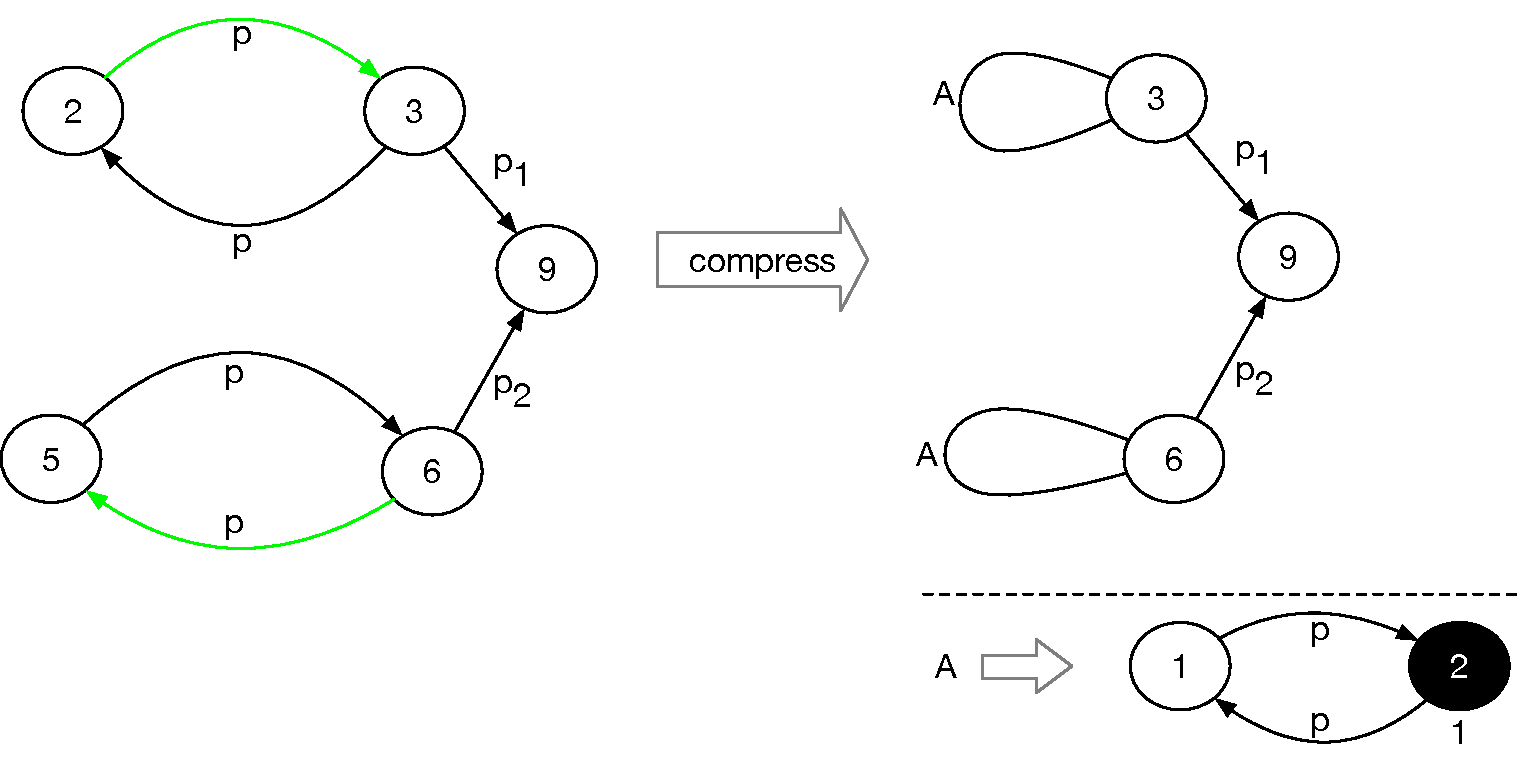
\includegraphics[width=0.9\textwidth]{figures/approach/symmetricMatEx2}
	\caption{A sub graph with the symmetric predicate $p$ (on the left side). The green edges have been added. Afterwards, two occurrences of the digram A can be found. The compressed graph is shown on the right side.}
	\label{fig:symDirectReplacement}
\end{figure}

\begin{figure}[h]
	\centering
	\subfloat[A sub graph to which the green edges were added. Two occurrences of the digram in Fig.~\ref{fig:symmetricMatDigram} are marked by red ovals.]{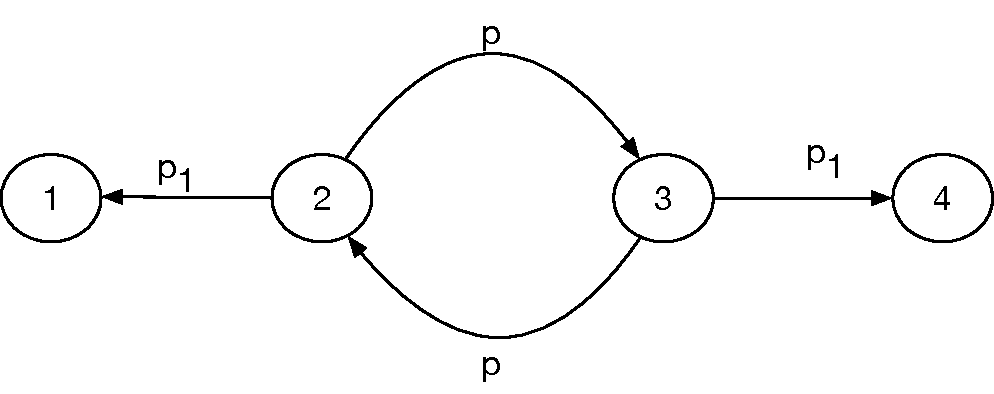
\includegraphics[width=0.45\textwidth]{figures/approach/symmetricMat}\label{fig:symmetricMat}}
	\hfill
	\subfloat[The digram that can be found twice in the graph of Fig.~\ref{fig:symmetricMat} after the green edges were added.]{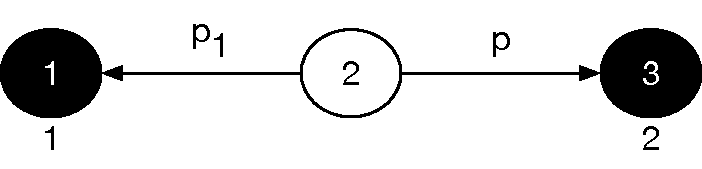
\includegraphics[width=0.45\textwidth]{figures/approach/symmetricMatDigram}\label{fig:symmetricMatDigram}}
	\caption{Visualization of the benefits of adding symmetric edges to the graph. $p$ is symmetric, all other properties are not.}
	\label{fig:symmetricMatIndirect}
\end{figure}

In Ch.~\ref{sec:relatedworkExDigramReplacement}, it was shown that more edges can also lead to a worse compression ratio, since internal nodes of a digram are not allowed to be connected to other nodes in the graph. So, it could be argued that adding symmetric edges makes GRP find less digram occurrences. But this is not the case, since the nodes, which the symmetric edges are added to, were already connected before. An example supporting this argument can be seen in Fig.~\ref{fig:symmetricMatIndirect}. In Fig.~\ref{fig:symmetricMat}, a graph is shown whereby $p$ is the only symmetric property. Hence, the green edges were added to the graph. Due to the addition, the digram of Fig.~\ref{fig:symmetricMatDigram} can be found twice, whereas it was previously found only once. So, the addition delivers a better compression potential here. At the same time, the degrees of  the nodes 2, 3, 5 and 6 are increased by one. But this should not decrease the probability of finding other digrams in the graph, since those nodes were already connected before.

The replacement of the digram in Fig.~\ref{fig:symmetricMatDigram} is not illustrated here, as that digram type was already explained in Ch.~\ref{sec:relatedworkExDigramReplacement}.



\subsubsection{Inverse Properties}\label{sec:approachInverse}

One property of~\cite{owl} is {\tt owl:inverseOf}, which is defined for two properties $p_1, p_2$. If $(s,p_1,o)$ exists then $(o,p_2,s)$ should also exist and vice versa. Analogously to {\tt owl:SymmetricProperty}, it can be the case that only one of the two triples is explicitly mentioned. It is reasonable to argue in a similar way for adding those edges to the graph here. It can decrease $ELR$ if there are many occurrences of a few inverse properties. Also, the added edges can directly produce a high number of digram occurrences which the two edges are part of (similar to Fig.~\ref{fig:symDirectReplacement}). Furthermore, it will not create an unfavorable graph structure, but enable GRP to find other digram occurrences (similar to Fig.~\ref{fig:symmetricMatIndirect}).


\subsubsection{Transitive Properties}\label{sec:approachTransitive}

In~\cite{owl}, a predicate can be denoted as transitive ({\tt owl:TransitiveProperty}). Let $p$ be transitive. If the triples $(1,p,2),(2,p,3)$ exist then $(1,p,3)$ should also exist. Consequently, this holds also for an arbitrarily long path from $1$ to $n$, as illustrated in Fig.~\ref{fig:transitiveMat}. Such a path, with the length of at least two, is called \tp from now on. If there exists a \tp between two nodes $i$ and $j$, then the edge $(i,j)$ is called \dtpp So, in Fig.~\ref{fig:transitiveMat}, the edges $(1,3)$ and $(1,n)$ are \dtpsp

\begin{figure}[h]
	\centering
	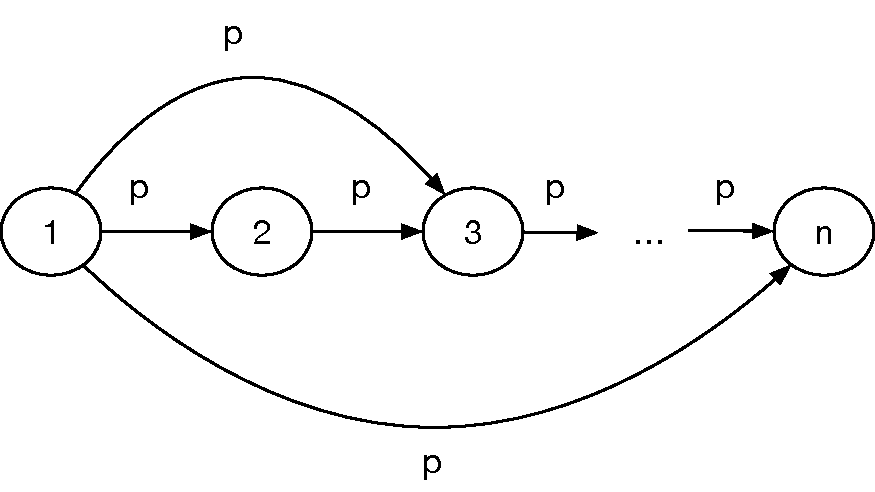
\includegraphics[width=0.5\textwidth]{figures/approach/transitiveMat}
	\caption{A sub graph with the transitive predicate $p$.}
	\label{fig:transitiveMat}
\end{figure}

The shown graph shall again be seen as some sub graph. The approach is to remove all \dtpsp This is reasonable, as it gives the nodes $i$ and $j$ a lower degree, and therefore GRP can have a higher chance to find other digrams in which those nodes are involved. An example is shown in Fig.~\ref{fig:transitiveMatExGraph} where the red dashed edges are removed. After that, two occurrences of the digram in Fig.~\ref{fig:transitiveMatExDigram} can be found. Before the removing those occurrences were not present, since the nodes 2 and 5 were connected to other nodes which is not allowed.

\begin{figure}[h]
	\centering
	\subfloat[A sub graph from which the red dashed edges were removed. Two occurrences of the digram in Fig.~\ref{fig:transitiveMatExDigram} are marked by red ovals.]{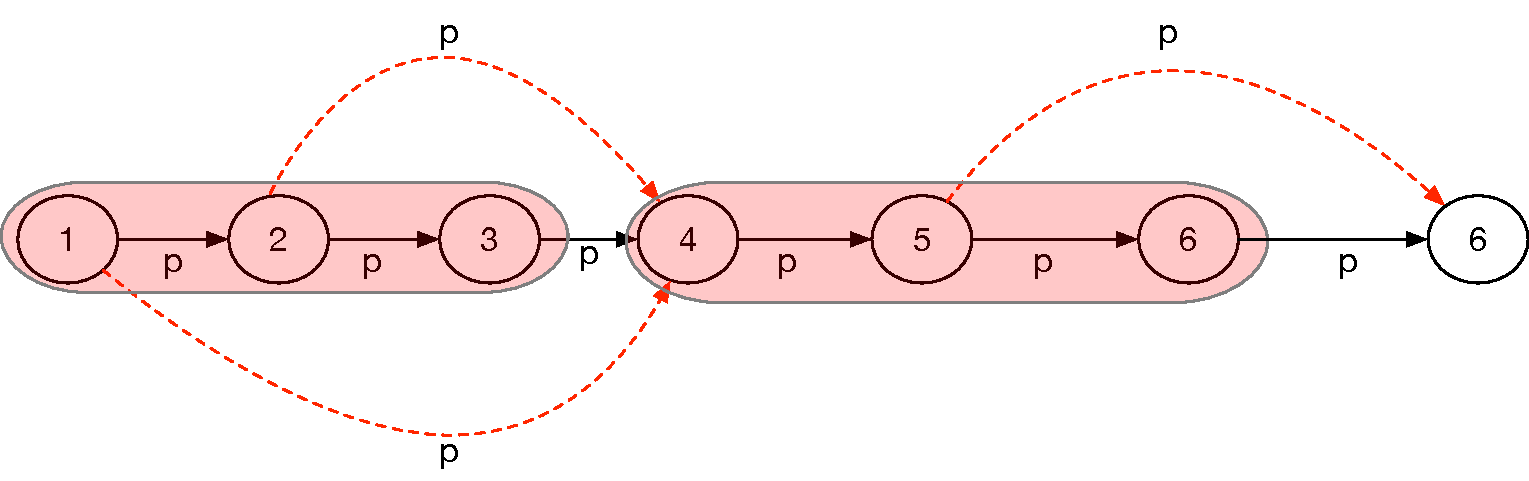
\includegraphics[width=0.9\textwidth]{figures/approach/transitiveMatEx}\label{fig:transitiveMatExGraph}}
	\hfill
	\subfloat[The digram that can be found twice in the graph of Fig.~\ref{fig:transitiveMatExGraph} after the red dashed edges were removed.]{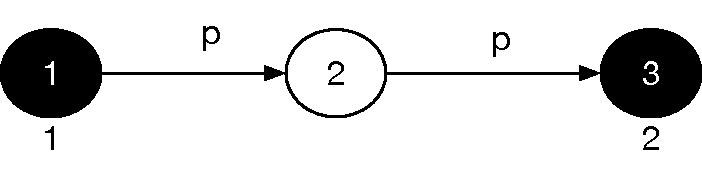
\includegraphics[width=0.45\textwidth]{figures/approach/transitiveMatExDigram}\label{fig:transitiveMatExDigram}}
	\caption{Visualization of the benefits of removing \dtps from the graph. $p$ is transitive.}
	\label{fig:transitiveMatEx}
\end{figure}

The opposing approach is to add all \dtpsp But a strong argument against this approach is that it would dramatically increase the number of edges, because for each pair $(i,j)$ (with $i,j\in \{1,...,n\} $  and distance between $i$ and $j$ greater than 1), an edge $(i,j)$ would be added. After increasing the graph's size so much it is unlikely that $out_{graph}$ becomes smaller even if more digrams could be found for some reason. 


\subsubsection{Equal Properties}\label{sec:approachEqualProperties}

Further properties of~\cite{owl} are {\tt owl:equivalentProperty} and {\tt owl:sameAs}. The first one denotes that two properties are equivalent, but that does not mean that they are equal. In contrast, the latter one is expressing equality. If there is a property $p$ which is equal to other properties $p_1,..,p_n$, then one approach could be to replace each occurrence of $p_1,..,p_n$ with $p$. This would reduce $ELR$ and, at the same time, not change the structure of the graph. However, this approach was not implemented, since the thesis focuses on compressing single RDF graphs and {\tt owl:sameAs} typically connects multiple graphs with each other. Compressing multiple graphs would lead to more complexity, because not only properties can be the same, but single nodes can be marked as the same as well.


\subsection{Dictionary Improvements}\label{sec:approachDictImprovements}


According to~\cite{hdt}, the dictionary ($out_{dict}$) makes up most of the memory of the complete output $out$. First results of Ch.~\ref{sec:evaluationHDTvsGRP} also show that. It is therefore worth investigating whether the dictionary can be compressed better. It can be taken advantage of certain features of the dictionary to achieve that. In order to do that we use $Dict_{HDT}$ as the basis and further improve it.

\subsubsection{Literals}\label{sec:approachLiterals}

Objects in RDF can be literals. Literals typically contain constant values and usually have no common prefixes. Therefore, the compression of \DHDT{} is not suitable for these. It would be possible to use different compression techniques for different types of data values (integer, double, string, etc.). The thesis will focus on compressing strings.

Since those strings can contain whole flow texts, a text compression would probably be well applicable. An example of such a text compression is a Huffman Code~\cite{huffman}. Here, every single character of a text is binary coded, whereby frequently occurring characters get short and rare characters get longer codes. These codes are expressed by a binary Huffman tree. An example can be seen in Fig.~\ref{fig:huffmantree}. Each leaf contains a symbol whereas the ones and zeros on the path to the symbol define its code. The tree is constructed in such a way that paths to frequent characters are shorter than those to rare characters. The whole procedure can be seen in~\cite{huffman}.

\begin{figure}
	\centering
	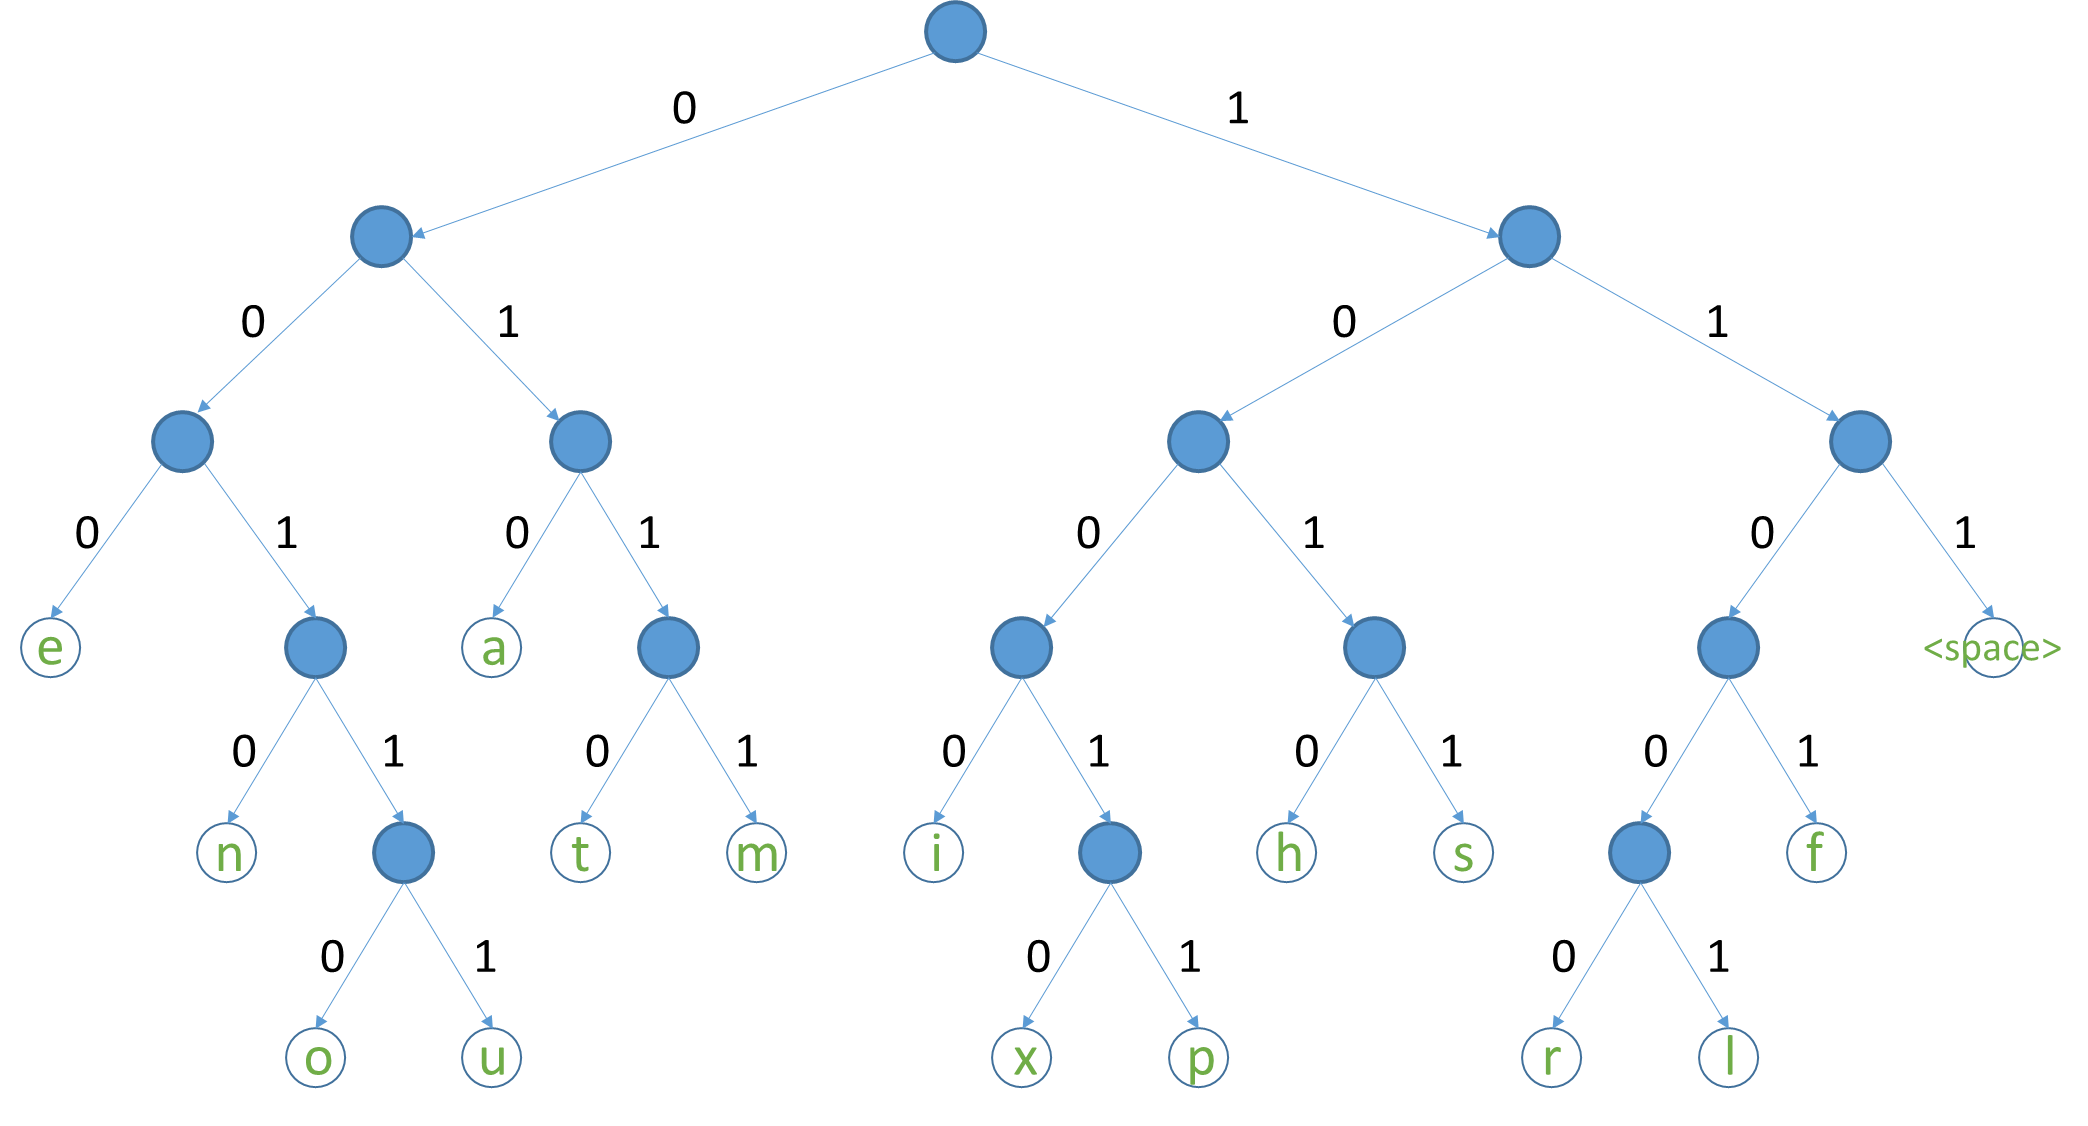
\includegraphics[width=0.9\linewidth]{figures/4_rdf_specific_features/huffman}
	\caption{An example of a Huffman Tree.}
	\label{fig:huffmantree}
\end{figure}

\subsubsection{Blank Nodes}\label{sec:approachBlankNodes}

As already mentioned in Ch.~\ref{sec:relatedworkRDF}, every blank node gets an ID. These IDs are usually chosen arbitrarily and have no meaning beyond that. When reading an RDF graph with the Jena-API~\footnote{\label{foot:5}https://jena.apache.org/index.html} (which is used by HDT according to~\cite{hdt}) random strings are assigned to the blank nodes, which are quite long. They also have no common prefixes, which makes \DHDT{} ineffective here. 

To improve the compression, the IDs of the blank nodes could be reassigned. For example, numbers from 1 to $n$ ($n=$ number of blank nodes) can be used to get short IDs. 

Another possibility is not to save the IDs of the blank nodes at all. In HDT all strings in the dictionary (including the blank node IDs) are mapped to short IDs. Thus, the blank node IDs are in principle already stored. They can therefore be removed from the dictionary. 















